\documentclass[12pt,twoside, a4paper, twocolumn]{article}
\usepackage[utf8]{inputenc}
\usepackage[brazil]{babel}
\usepackage[margin = 0.5in]{geometry}
\usepackage{amsmath}
\usepackage{amsthm}
\usepackage{amssymb}
\usepackage{amsthm}
\usepackage{setspace}
\usepackage[americanvoltages,fulldiodes,siunitx]{circuitikz}
\usepackage{lipsum}
\usepackage{pgfplots}
\usepackage{ifthen}
\usepackage{adjustbox}
\usepackage[section]{placeins}
\usepackage{hyperref}
\usepackage{graphicx}


\graphicspath{ {./images/} }
\pgfplotsset{compat=newest}



%  #1 color - optional #2 x_0 #3 y_0 #4 x_f #5 y_f #6 name - optional  #7 true if adding lines to axis

\newcommand{\drawvector} [9] [color=cyan] {
    \draw[line width=1.5pt,#1,-stealth](axis cs: #2, #3)--(axis cs: #4, #5) node[anchor=south west]{$#6$};

    

\ifthenelse{\equal{#7}{true}}{
    \draw[line width=1pt,#1, dashed](axis cs: #4, #5)--(axis cs: #4, 0) node[anchor= north west]{$#8$};
    \draw[line width=1pt,#1, dashed](axis cs: #4, #5)--(axis cs: 0, #5) node[anchor=south east]{$#9$};
    }
    {}
}

\newcommand\deriv[2]{\frac{\mathrm d #1}{\mathrm d #2}}


\title{Primeiro Relatorio de Fisica Experimental 2}
\author{Henrique da Silva \\ hpsilva@proton.me}
\date{\today}
\pgfplotsset{width = 10cm, compat = 1.9}


\begin{document}
\maketitle
\pagenumbering{gobble}
\newpage
%pagenumbering{roman}
\tableofcontents
\newpage

\section{Introdução}

\paragraph*{Neste relatório, vamos discutir um objeto se movendo sobre uma superficie com atrito e suas grandezas relacionadas}

\paragraph*{Todos arquivos utilizados para criar este relatorio, e o relatorio em si estao em:  \url{https://github.com/Shapis/ufpe_ee/tree/main/4th semester/}}

\section{Tarefas}

\subsection{Grafico de $d$ em funcao de $v_0$}



\begin{adjustbox}{scale=0.75}
    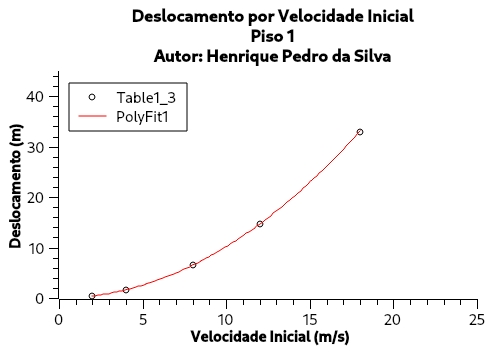
\includegraphics{Grafico-0.jpg}
\end{adjustbox}

\subsection{Esimacao visual}

\subparagraph*{Estimando visualmente a partir do grafico acima, podemos estimar o deslocamento $d$ como o seguinte:}

\begin{equation}
    \begin{aligned}
        v_0 = 15 m/s & \rightarrow d = 23.2 m \\
        v_0 = 21 m/s & \rightarrow d = 44.2 m \\
    \end{aligned}
\end{equation}

\subsection{Grafico de $d$ em funcao de $v_0^2$}



\begin{adjustbox}{scale=0.75}
    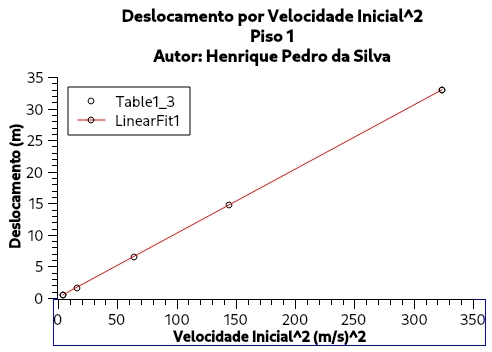
\includegraphics{Grafico-1.jpg}
\end{adjustbox}

\subsection{Relacao matematica entre $d$ e $v_0^2$}

\subparagraph*{Podemos observar que ha uma relacao linear entre $d$ e $v_0^2$, e tentando um \emph{fit} pelo SciDAVis conseguimos o seguinte: }

\begin{equation}
    d = 0.102 * V_0^2
\end{equation}

\subsection{Verificacao dos outros pisos}

\begin{adjustbox}{scale=0.75}
    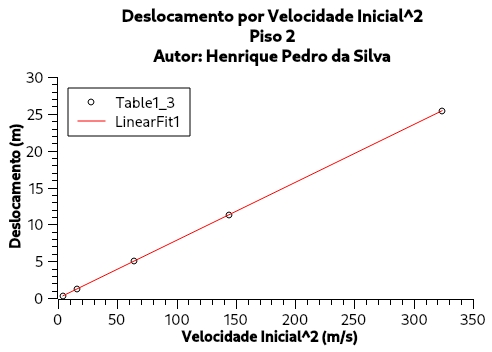
\includegraphics{Grafico-2.jpg}
\end{adjustbox}
\subparagraph*{}
\begin{adjustbox}{scale=0.75}
    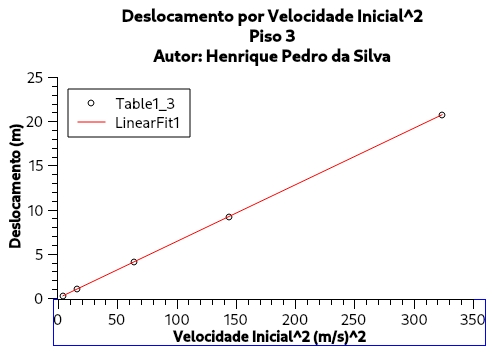
\includegraphics{Grafico-3.jpg}
\end{adjustbox}
\subparagraph*{}
\begin{adjustbox}{scale=0.75}
    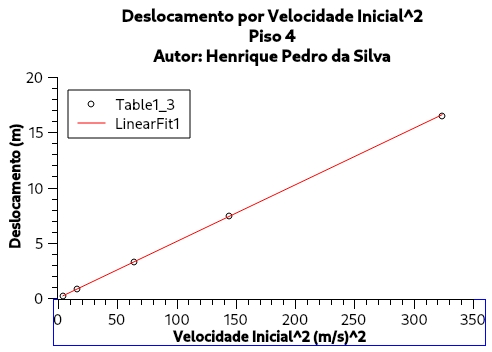
\includegraphics{Grafico-4.jpg}
\end{adjustbox}

\subparagraph*{Novamente fazendo \emph{fit} pelo SciDAVis conseguimos o seguinte:}

\begin{equation}
    \begin{aligned}
        Piso\, 1 & \rightarrow d = 0.102 * V_0^2 \\
        Piso\, 2 & \rightarrow d = 0.102 * V_0^2 \\
        Piso\, 3 & \rightarrow d = 0.102 * V_0^2 \\
        Piso\, 4 & \rightarrow d = 0.102 * V_0^2 \\
    \end{aligned}
\end{equation}

\subparagraph*{Notamos que a relacao continuar linear para todo tipo de piso.}


\paragraph*{\\ \\ \\ \\ \\ \\ \\ }

\subsection{Verificacao por grafico di-log}
\begin{adjustbox}{scale=0.70}
    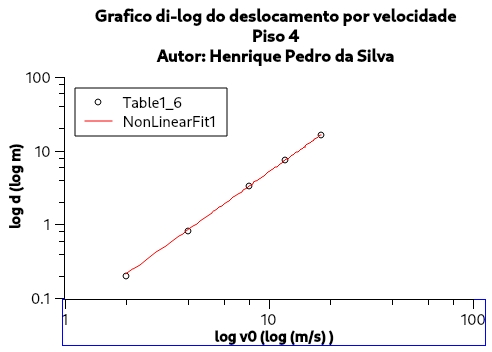
\includegraphics{Grafico-5.jpg}
\end{adjustbox}

\subparagraph*{Tinhamos como valor esperado $n = 2$, e por um \emph{fit} feito pelo SciDAVis conseguimos este como 1.983. Que esta bastante proximo do resultado esperado.}
\subparagraph*{Logo podemos considerar que de fato, ha uma relacao quadratica entre a velocidade inicial $V_0$ e o deslocamento $d$.}

\subsection{Deslocamento $d$ em funcao de velocidade inicial $v_0$}

\subparagraph*{Temos que a forca de atrito eh dada por}

\begin{equation}
    \begin{aligned}
        F = \mu * N = \mu * m * g
    \end{aligned}
\end{equation}

\subparagraph*{Inserindo isso na segunda lei de Newton teremos:}

\begin{equation}
    \begin{aligned}
         & F      = m*a \\
         & u*m*g  = m*a \\
         & u*g    = a
    \end{aligned}
\end{equation}

\subparagraph*{Tambem temos que:}

\begin{equation}
    \begin{aligned}
        V_f^2 = V_0^2 + 2*a*d \\
    \end{aligned}
\end{equation}

\subparagraph*{E como nosso $V_f$ eh 0, e nosso atrito sempre se opoe ao movimento podemos simplificar e re-escrever como:}

\subparagraph*{Tambem temos que:}

\begin{equation}
    \begin{aligned}
        0 & = V_0^2 - 2*a*d     \\
        d & = \frac{V_0^2}{2*a} \\
    \end{aligned}
\end{equation}

\subparagraph*{Agora substituindo (5) em (7) finalmente temos uma equacao que relaciona $d$ $\mu$ e $V_i$}

\begin{equation}
    \begin{aligned}
        d  = \frac{V_0^2}{2*\mu*g} \\
    \end{aligned}
\end{equation}

\subsection{Obtendo $\mu$ para os pisos}

\subparagraph*{Agora vamos utilizar a relacao que descobrimos entre $\mu$ $d$ e $V_0$ para conseguir um $\mu$ para cada piso}

\subparagraph*{Tinhamos que ha uma relacao linear entre $d$ e $V_0^2$ que tinha forma de:}

\begin{equation}
    \begin{aligned}
        d = A * V_0^2 \\
    \end{aligned}
\end{equation}

\subparagraph*{Podemos entao substituir isto no nosso (8)}

\begin{equation}
    \begin{aligned}
        A * V_0^2         & = \frac{V_0^2}{2*\mu*g} \\
        \frac{1}{2*\mu*g} & = A                     \\
        \mu               & = \frac{1}{A*g*2}       \\
        \mu               & = \frac{1}{A*9.8*2}     \\
    \end{aligned}
\end{equation}

\subparagraph*{Com a equacao (10) em maos e utilizando os valores obtidos em (3) teremos o seguinte:}

\begin{equation}
    \begin{aligned}
        \mu \, do \, Piso\, 1 & \rightarrow 0.500 \\
        \mu \, do \, Piso\, 2 & \rightarrow 0.654 \\
        \mu \, do \, Piso\, 3 & \rightarrow 0.810 \\
        \mu \, do \, Piso\, 4 & \rightarrow 1.020 \\
    \end{aligned}
\end{equation}

\section{Conclusao}

\subparagraph*{Observei que ha uma relacao quadratica entre o deslocamento e a velocidade inicial de lancamento.   }

\subparagraph*{Tambem que a massa nao importa.}

\subparagraph*{As unicas coisas que importam para o deslocamento sao a velocidade inicial, a gravidade, e o coeficiente de atrito.}

\subparagraph*{E nenhum desses fatores altera o fato da relacao ser quadratica.}

\subparagraph*{Vi tambem que posso fazer ajuste de dados de varias maneiras com o SciDAVis.}

\subparagraph*{E posso deduzir numericamente relacoes que nao seriam tao triviais de deduzir analiticamente.}

\end{document}

